\documentclass[12pt]{article}
\usepackage{graphicx}

\begin{document}
\graphicspath{ {./} }

\section{Use Case}
I chose last semester's final experiment from the lecture "Data Oriented Programming Paradigm".

\subsection{Experiment Task Description}
The goal of this project is to answer the following question related to country-scale extreme poverty: \newline
    Question: What are the most predictive features for countries living in extreme poverty?

\subsection{Methodology}
In order to answer this question, we considered the data available from Unesco's Institute for Statistics. UNESCO had its own data set labeled "Demographic and socio-economic", which contained socio-economic information about all the countries in the world going back to the 1970s.
We then proceeded to create linear predictive models using python's sci-kit learn and visualized the feature importance for the prediction models. \newline
We concluded, that Fertility Rate was the most important feature for predicting countries in extreme poverty followed by Population Growth, Life Expectancy, Mortality and Percentage living in rural areas. \newline
The experiment is further explainde in the flowchart diagram in Figure 1. \newline
The Visualization of the results can be seen in figure 2.


\begin{figure}[h]
    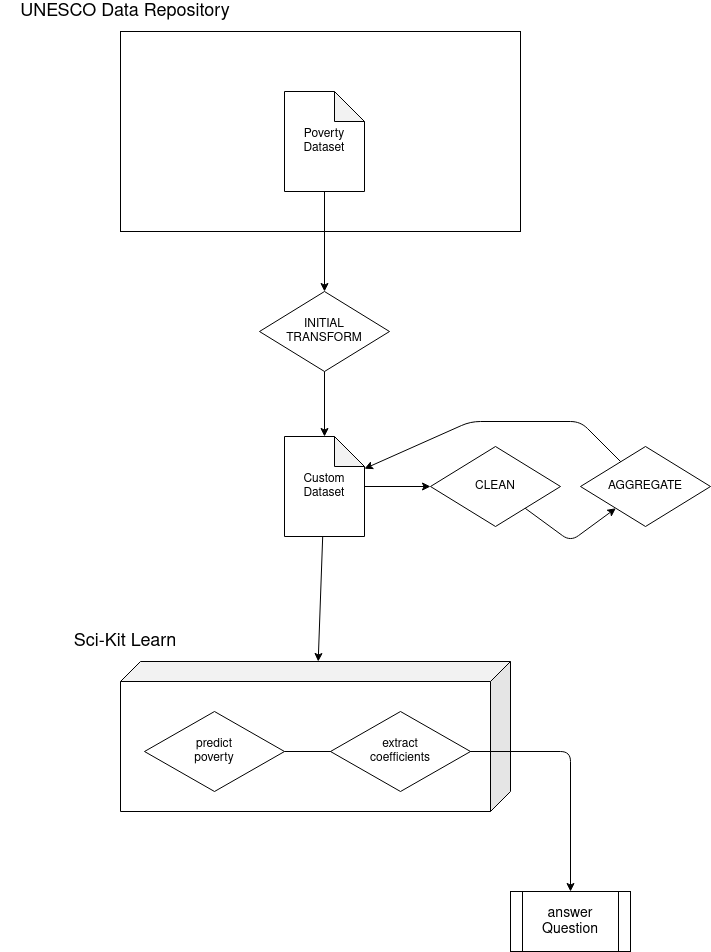
\includegraphics[scale=0.5]{DS1.png}
    \caption{Experiment Workflow}
\end{figure}

\begin{figure}[h]
    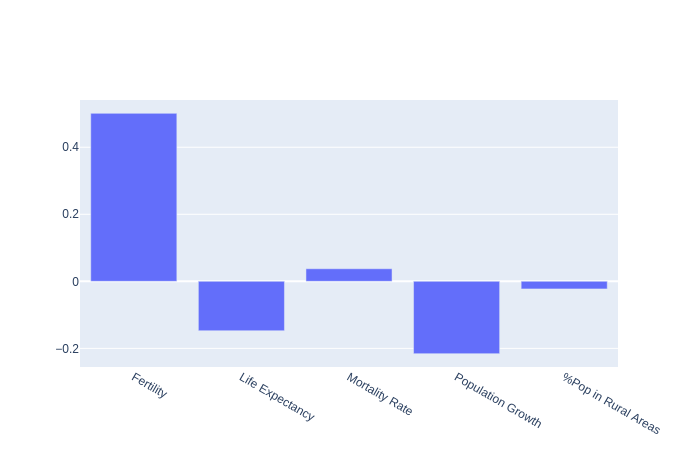
\includegraphics[scale=0.65]{feature_importances.png}
    \caption{Relative Feature Importance}
\end{figure}



\end{document}